\documentclass{article}
\usepackage {graphicx}
\begin{document}
\title{Machine, Data and Learning: Assignment 1}
\author{Shubhangi Dutta (2018113004), Rishav Kundu (2019121007)}
\maketitle
\newpage
\section{Q1}
\subsection{Bias and Variance table for Polynomial Fit}

\begin{center}
\begin{tabular}{ | c | c | c | }
\hline
Degree & Bias & Variance \\ 
\hline \hline
1 & 30.37408273224508 & 0.09341804232251934 \\ 
\hline
2 & 6.36517276002383 & 0.02342602657696328 \\ 
\hline
3 & 5.2694201717911 & 0.032432266902508056 \\ 
\hline
4 & 3.1505752052574882 & 0.024700107894447286 \\ 
\hline
5 & 2.929418757965218 & 0.026853397616000967 \\ 
\hline
6 & 2.5924918432950887 & 0.025693386573740703 \\ 
\hline
7 & 2.4297943137364473 & 0.03185979691247053 \\ 
\hline
8 & 2.401411060979298 & 0.04025175952926954 \\ 
\hline
9 & 2.4046636467383133 & 0.042469600227830584 \\ 
\hline
10 & 2.417341604358687 & 0.047025847634951844 \\ 
\hline
11 & 2.2129311318120677 & 0.039547099980470186 \\ 
\hline
12 & 2.212837336615444 & 0.040014205734798594 \\ 
\hline
13 & 2.04333525171306 & 0.04465927459234133 \\ 
\hline
14 & 2.044422212520452 & 0.054205383136040355 \\ 
\hline
15 & 2.048575476047638 & 0.05184750688113316 \\ 
\hline
16 & 2.055511225205248 & 0.05780882443374418 \\ 
\hline
17 & 1.5676562220889405 & 0.041844397410982295 \\ 
\hline
18 & 1.580772918328726 & 0.04997588536630306 \\ 
\hline
19 & 1.5753515315568343 & 0.04587184307778622 \\ 
\hline
20 & 1.5700026631879862 & 0.05801091925152769 \\ 
\hline
21 & 1.0749491166688236 & 0.09679378957868845 \\ 
\hline
22 & 1.0773198062251255 & 0.11390297913298957 \\ 
\hline
23 & 1.0665098885278717 & 0.11908804588652822 \\ 
\hline
24 & 0.9482893416038309 & 0.06419302845892338 \\ 
\hline
25 & 0.8195925886965155 & 0.04129120796111043 \\
\hline 
26 & 0.48111794650702805 & 0.14104241519819197 \\ 
\hline
27 & 0.5641635223612983 & 0.12850830831675497 \\ 
\hline
28 & 0.6162690155838716 & 0.11799193084262229 \\ 
\hline
29 & 0.15763860143872435 & 0.11608161243502352 \\ 
\hline
30 & 0.136425684845244 & 0.04422191964882733 \\ 
\hline
\end{tabular}
\end{center}

\subsection{Bias-Variance Vs Degree Plot for Polynomials Degree 1-9}
\subsubsection{Plot}
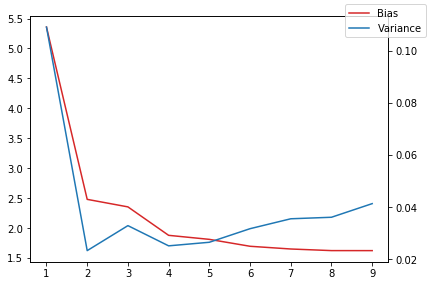
\includegraphics[scale=.9]{images/1-9.png}
\subsubsection{Observations and Analysis}
\begin{itemize}
\item Both bias and variance are very large for the linear fit. The model is underfit and performs poorly for the given data.
\item For higher degrees ($>$ 1, $<$ 6), both bias and variance decrease. The models are better fit to the data points, so both decrease.
\item Variance increases again for even higher degree polynomials (>6) but it is not significant compared to the drop between degree  1 and 2. The model is overfitting, and hence is not a good fit for the test data and is accounting for small deviations, making variance high.
\end{itemize}
\subsection{Bias-Variance Vs Degree Plot for Polynomials Degree 2-9}
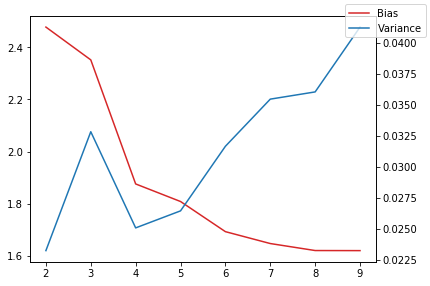
\includegraphics[scale=.9]{images/2-9.png}
\subsubsection{Observations and Analysis}
\begin{itemize}
\item Bias is high but variance is low for the degree 2 fit. The model is underfit and performs poorly for the test data.
\item For higher degrees ($>$ 2, $<$ 5), both bias and variance decrease. The models are better fit to the data points, so both decrease.
\item The intersection point is at the 5 degree polynomial. Both bias and variance are low and this is optimal fit.
\item Variance increases again for even higher degree polynomials (>6) and it is significant compared to the drop in bias. The model is overfitting, and hence is not a good fit for the test data and is accounting for small deviations, making variance high.
\end{itemize}
\subsection{Bias-Variance Vs Degree Plot for Polynomials Degree 1-30}
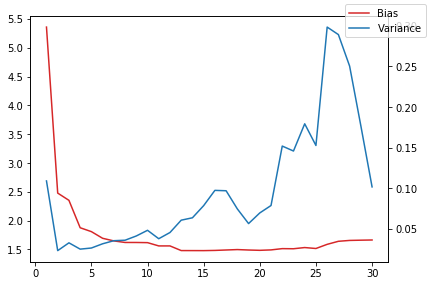
\includegraphics[scale=.9]{images/1-30.png}
\subsubsection{Observations and Analysis}
\begin{itemize}
\item Both bias and variance are very large for the linear fit. The model is underfit and performs poorly for the given data.
\item For higher degrees ($>$ 1, $<$ 10), both bias and variance decrease. The models are better fit to the data points, so both decrease.
\item The intersection point is at the 5 degree polynomial. Both bias and variance are low and this is optimal fit.
\item Variance increases again sharply for even higher degree polynomials (>10). Bias keeps reducing in approximately linear way. The model is overfitting, and hence is not a good fit for the test data and is accounting for small deviations, making variance high. 
\item In some cases, such as at degree 24-25 and again at 30. In these cases, the model incidentally fit well, probably due to the nature of the data.
\end{itemize}

\section{Q2}
\subsection{Bias and Variance table for Polynomial Fit}


\end{document}
